\documentclass{article}

\usepackage[preprint]{neurips_2026}

\makeatletter
\renewcommand{\@notice}{}
\makeatother

\usepackage[utf8]{inputenc}
\usepackage[T1]{fontenc}
\usepackage{amsmath}
\usepackage{amssymb}
\usepackage{booktabs}
\usepackage{array}
\usepackage{graphicx}
\usepackage{adjustbox}
\usepackage{caption}
\usepackage{float}
\usepackage{placeins}
\usepackage{xcolor}
\usepackage{hyperref}
\usepackage{url}

\hypersetup{
  colorlinks=true,
  linkcolor=blue,
  citecolor=blue,
  urlcolor=blue
}

\raggedbottom
\setlength{\textfloatsep}{7pt plus 2pt minus 2pt}
\setlength{\intextsep}{7pt plus 2pt minus 2pt}
\setlength{\floatsep}{6pt plus 2pt minus 2pt}
\renewcommand{\topfraction}{0.97}
\renewcommand{\bottomfraction}{0.90}
\renewcommand{\textfraction}{0.03}
\renewcommand{\floatpagefraction}{0.88}
\setcounter{topnumber}{5}
\setcounter{bottomnumber}{4}
\setcounter{totalnumber}{9}
\captionsetup{font=small,skip=3pt}

\newcommand{\pct}{\%\ }
\newcommand{\Ahat}{\ensuremath{\hat{A}}}

\title{Assignment 3 Report: Graph Neural Networks for Traffic Forecasting on LargeST-SD}

\author{
  Daniyal Hussain Shah
}

\begin{document}

\maketitle

\begin{abstract}
This report studies how graph structure supplies information to a spatio-temporal forecaster. Questions 1 and 2 use small road-sensor examples. A sum aggregator with affine messages keeps only the neighbour count and total trend, while a base-$(K{+}1)$ message makes the sum a lossless code for all three trend counts. A layer that treats both ring neighbours alike cannot represent motion; separate directional weights or one step of history make the moving pattern exactly predictable. Questions 3 to 7 forecast one hour of traffic flow for the 716 San Diego sensors of LargeST from two hours of history. A lightweight model with a temporal convolution encoder, one graph convolution layer, and a linear forecast head reduces test MAE from 24.20 for the temporal-only baseline to 23.17 with the fixed road graph, 20.91 with a learned adjacency, and 21.73 with a hybrid graph. The learned graph forecasts best but is not geographic: its strongest edges are road edges no more often than random sensor pairs, although they link sensors whose local fluctuations are correlated. Two implementation details proved necessary for valid comparisons: a residual path around the graph layer and the exclusion of learned-graph embeddings from weight decay. Code, results, and instructions are available at \url{https://github.com/syeddaniyalg/cs434-pa3}.
\end{abstract}

\section{Introduction}

A graph neural network can use only the information that its messages and aggregation preserve. If the aggregation discards a quantity, no later layer can recover it. If the graph connects the wrong sensors, or connects them without direction, the model cannot represent how congestion moves. This report first studies these limits on small examples where the answer can be proved and checked exactly. It then measures the same issues on a real forecasting task: the San Diego subset of LargeST~\citep{liu2023largest}, with a fixed road graph, a learned graph, and their combination.

Every numerical claim in this report is produced by the submitted code. Results for Questions 1 and 2 are verified by exhaustive enumeration or random substitution. Results for Questions 3 to 6 use one fixed seed and the same training protocol for every model.

\section{Question 1: What Does a Sum Remember?}
\label{sec:q1}

\subsection*{Q1(a): Affine messages}

With $\phi(x)=wx+c$, the aggregated message is
\begin{equation}
  \sum_{u\in\mathcal{N}(v)}\left(w x_u+c\right)=w\,S_v+c\,n_v .
\end{equation}
The layer output is $h_v=\rho(wS_v+cn_v)$. Two neighbourhoods with equal $n_v$ and equal $S_v$ give the same argument to $\rho$ for every $w$ and $c$, so they give the same output for every $\rho$. The neighbourhoods $\{-1,+1\}$ and $\{0,0\}$ both have $n_v=2$ and $S_v=0$, but the first has no steady neighbours and the second has two. No choice of $w$, $c$, or $\rho$ can separate them. The check script confirms equal aggregates for five random $(w,c)$ pairs.

\subsection*{Q1(b): A lossless scalar message}

Let $B=K+1$ and choose
\begin{equation}
  \phi(-1)=1,\qquad \phi(0)=B,\qquad \phi(+1)=B^2 .
\end{equation}
If a neighbourhood has $a$ slowing, $b$ steady, and $c$ speeding-up neighbours, the sum is $s=a+bB+cB^2$. Each count is at most $K<B$, so $a$, $b$, and $c$ are the three digits of $s$ in base $B$. No digit can carry into the next place value. The counts are recovered by
\begin{equation}
  a=s \bmod B,\qquad b=\lfloor s/B\rfloor \bmod B,\qquad c=\lfloor s/B^2\rfloor .
\end{equation}
For $K=8$ the messages are $(1,9,81)$. All 164 count triples with $1\le a+b+c\le 8$ give 164 distinct sums, the largest being 648, and the decoder returns every triple exactly. Base $K=8$ is too small: the triples $(0,0,1)$ and $(0,8,0)$ both sum to 64. To count only non-steady neighbours, $\phi(x)=x^2$ suffices, because it maps $\pm1$ to 1 and 0 to 0, so the sum equals $a+c$ for any neighbourhood size.

\subsection*{Q1(c): Sum, mean, and max}

Table~\ref{tab:q1c} lists the result for each task and aggregator. The script enumerates all 164 allowed neighbourhoods and searches for two neighbourhoods with the same aggregated vector but different answers. If none exists, it verifies the stated rule on every neighbourhood.

\begin{table}[htbp]
\centering
\caption{Aggregator comparison with one-hot messages. $s_k$, $m_k$, and $\max_k$ denote coordinate $k$ of the sum, mean, and max (1: slowing, 2: steady, 3: speeding up).}
\label{tab:q1c}
\footnotesize
\begin{adjustbox}{max width=\linewidth}
\begin{tabular}{>{\raggedright\arraybackslash}p{0.21\linewidth}lc>{\raggedright\arraybackslash}p{0.56\linewidth}}
\toprule
Task & Method & Possible? & Reason \\
\midrule
(i) Count steady & Sum & Yes & $\rho$ returns $s_2$. \\
 & Mean & No & $\{0\}$ and $\{0,0\}$ both give $(0,1,0)$; the answers are 1 and 2. \\
 & Max & No & The same pair gives $(0,1,0)$; the answers are 1 and 2. \\
\midrule
(ii) More than half slowing & Sum & Yes & $s_1>(s_1+s_2+s_3)/2$, which is equivalent to $s_1>s_2+s_3$. \\
 & Mean & Yes & $m_1>1/2$. \\
 & Max & No & $\{-1,+1\}$ and $\{-1,-1,+1\}$ both give $(1,0,1)$; the answers are No and Yes. \\
\midrule
(iii) Any slowing & Sum & Yes & $s_1>0$. \\
 & Mean & Yes & $m_1>0$. \\
 & Max & Yes & $\max_1=1$. \\
\bottomrule
\end{tabular}
\end{adjustbox}
\end{table}

The pattern follows from what each aggregator keeps. The sum keeps the counts. The mean keeps the proportions but loses the neighbourhood size, so it fails only for the count task. The max keeps only which trends are present, so it answers the existence task and nothing else.

\section{Question 2: Which Way Is the Slowdown Moving?}
\label{sec:q2}

\subsection*{Q2(a): A layer that treats both neighbours alike}

\paragraph{(i) Least-squares fit.}
With a single slowdown at sensor 20, every sensor other than 19, 20, and 21 receives prediction zero and target zero. The three remaining predictions and targets are
\begin{equation}
  (\hat x_{19},\hat x_{20},\hat x_{21})=(b,\,a,\,b),\qquad (x_{19},x_{20},x_{21})(t+1)=(1,\,0,\,0).
\end{equation}
The squared error is $(b-1)^2+a^2+b^2$. Setting both derivatives to zero gives $a=0$ and $b=1/2$, with minimum error $0.5$. A numerical least-squares fit returns the same values. The symmetric layer cannot place the slowdown at sensor 19 without placing the same amount at sensor 21, so it splits the mass equally.

\paragraph{(ii) Repeated application.}
Figure~\ref{fig:q2} compares 20 steps of the fitted layer with the true motion from the bump $x_i(0)=e^{-(i-20)^2/8}$. The true pattern moves one sensor per step and reaches sensor 0 at $t=20$ with unchanged peak height. The fitted layer keeps the pattern centred at sensor 20 and only diffuses it: the peak falls from 1.00 to 0.66 at $t=5$ and to 0.40 at $t=20$, while the number of sensors above $10^{-3}$ grows from 15 to 33. Total mass is preserved because $a+2b=1$, but the motion is lost.

\begin{figure}[htbp]
\centering
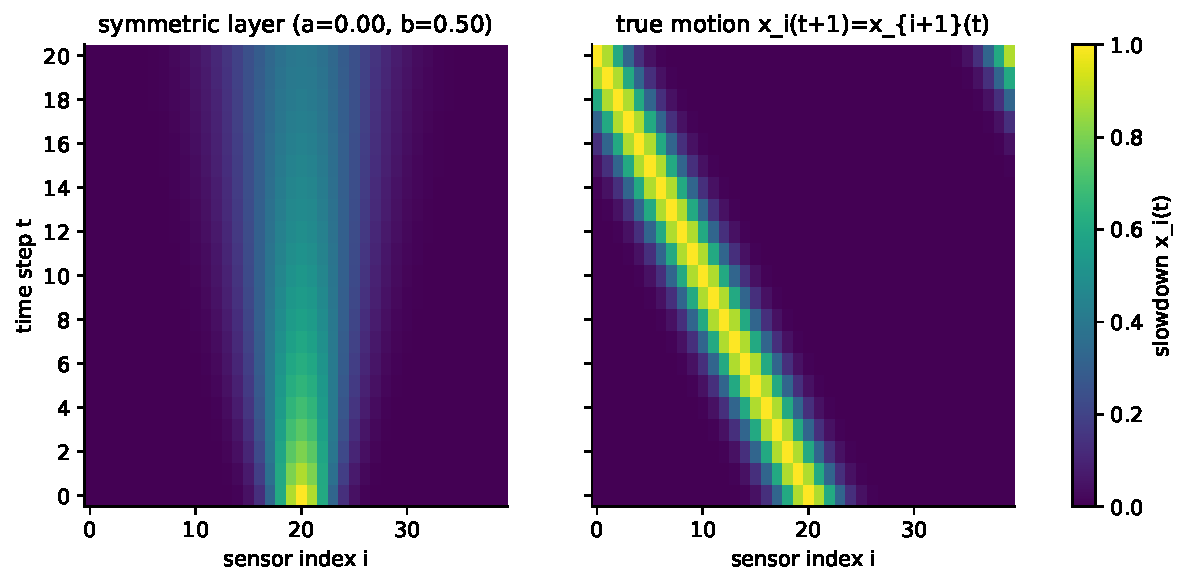
\includegraphics[width=0.92\linewidth]{figures/fig_q2_ring.pdf}
\caption{Twenty steps of the fitted symmetric layer ($a=0$, $b=0.5$) and of the true backward motion, on the same colour scale.}
\label{fig:q2}
\end{figure}

\subsection*{Q2(b): Directional weights}

Choose $a=0$, $w_-=0$, and $w_+=1$. Substitution gives $\hat x_i(t+1)=x_{i+1}(t)$, which is the motion rule itself, so the prediction is exact for every input. The difficulty in (a) disappears because the layer is told which neighbour lies ahead. In (a) the two neighbours share one weight, so any input that is mirror-symmetric about a sensor produces a mirror-symmetric prediction. With separate weights the layer can copy from the downstream side only.

As a 1D convolution, the kernel that multiplies $[x_{i-1},x_i,x_{i+1}]$ is $[w_-,a,w_+]=[0,0,1]$, applied as a cross-correlation as in PyTorch. The ring boundary is handled with circular padding of one sensor on each side, so sensor 39 reads sensor 0. The script confirms zero error for 200 random snapshots, both by direct substitution and with \texttt{conv1d} on circularly padded input.

\subsection*{Q2(c): Equal spatial weights with history}

\paragraph{(i) Backward motion.}
Choose $a=0$, $b=1$, and $c=-1$. Under $x_j(t)=x_{j+1}(t-1)$, the reading that was at sensor $i$ at time $t-1$ is now at sensor $i-1$, so $x_i(t-1)=x_{i-1}(t)$. Substitution gives
\begin{equation}
  \hat x_i(t+1)=x_{i-1}(t)+x_{i+1}(t)-x_{i-1}(t)=x_{i+1}(t)=x_i(t+1).
\end{equation}

\paragraph{(ii) Forward motion.}
Under $x_i(t+1)=x_{i-1}(t)$, the previous reading satisfies $x_i(t-1)=x_{i+1}(t)$. The same coefficients give
\begin{equation}
  \hat x_i(t+1)=x_{i-1}(t)+x_{i+1}(t)-x_{i+1}(t)=x_{i-1}(t)=x_i(t+1).
\end{equation}
The coefficients from (i) remain exact. A least-squares fit on 200 random pairs recovers $(0,1,-1)$ for both directions, and the maximum error is below $10^{-15}$.

\paragraph{(iii) Why history helps.}
The previous reading at sensor $i$ has moved to the neighbour in the direction of travel. Subtracting it cancels exactly that neighbour and leaves the neighbour behind sensor $i$, from which the pattern arrives next. The spatial weights stay equal, so the layer still has no notion of left or right. Direction is instead read from time: comparing the current and previous snapshots reveals which neighbour now holds the old reading. This is the same reason a temporal encoder can supply direction to a graph layer whose edges are undirected.

\section{Dataset Preparation and Graph Construction}
\label{sec:q3}

\subsection*{Q3(a): Data extraction and resampling}

The San Diego subset is defined as the 716 sensors in Caltrans District 11 of the LargeST metadata. Their 5-minute flow series for 2020 and 2021 are read from the raw LargeST files, giving 210,528 timestamps per sensor. LargeST flow is a vehicle count per 5-minute interval. Three consecutive readings are averaged, so each 15-minute value remains in vehicles per 5 minutes, which is the unit used by the LargeST benchmark. Summation would report vehicles per 15 minutes and would multiply every error by three. The result has 70,176 timestamps from 2020-01-01 00:00 to 2021-12-31 23:45.

\begin{table}[htbp]
\centering
\caption{Missing data and flow statistics after resampling.}
\label{tab:missing}
\footnotesize
\begin{tabular}{lr}
\toprule
Quantity & Value \\
\midrule
Missing rate, 5-minute / 15-minute & 5.07\pct / 5.06\% \\
Missing rate, train / validation / test (15-minute) & 4.09\pct / 6.07\pct / 6.01\% \\
Sensors with no observation in 2020 and 2021 & 19 \\
Sensors with more than 10\pct missing & 45 \\
Median per-sensor missing rate & 0.011\% \\
Timestamps with every sensor missing (15-minute) & 8 \\
Observed flow mean / standard deviation / maximum & 217.7 / 168.5 / 999 \\
\bottomrule
\end{tabular}
\end{table}

Table~\ref{tab:missing} summarises the missing data. Averaging uses only the readings available within each 15-minute bin, which removes most isolated 5-minute gaps. Remaining gaps are forward-filled, so a filled value never uses a later observation. Leading gaps are filled with the sensor's training mean. Every filled value is recorded in a mask and excluded from the loss and from all reported metrics. The 19 sensors that are never observed therefore contribute inputs but no targets. Figure~\ref{fig:q3week} shows one week for three sensors chosen at the 10th, 50th, and 90th percentiles of mean flow among sensors with less than 5\pct missing data.

\begin{figure}[htbp]
\centering
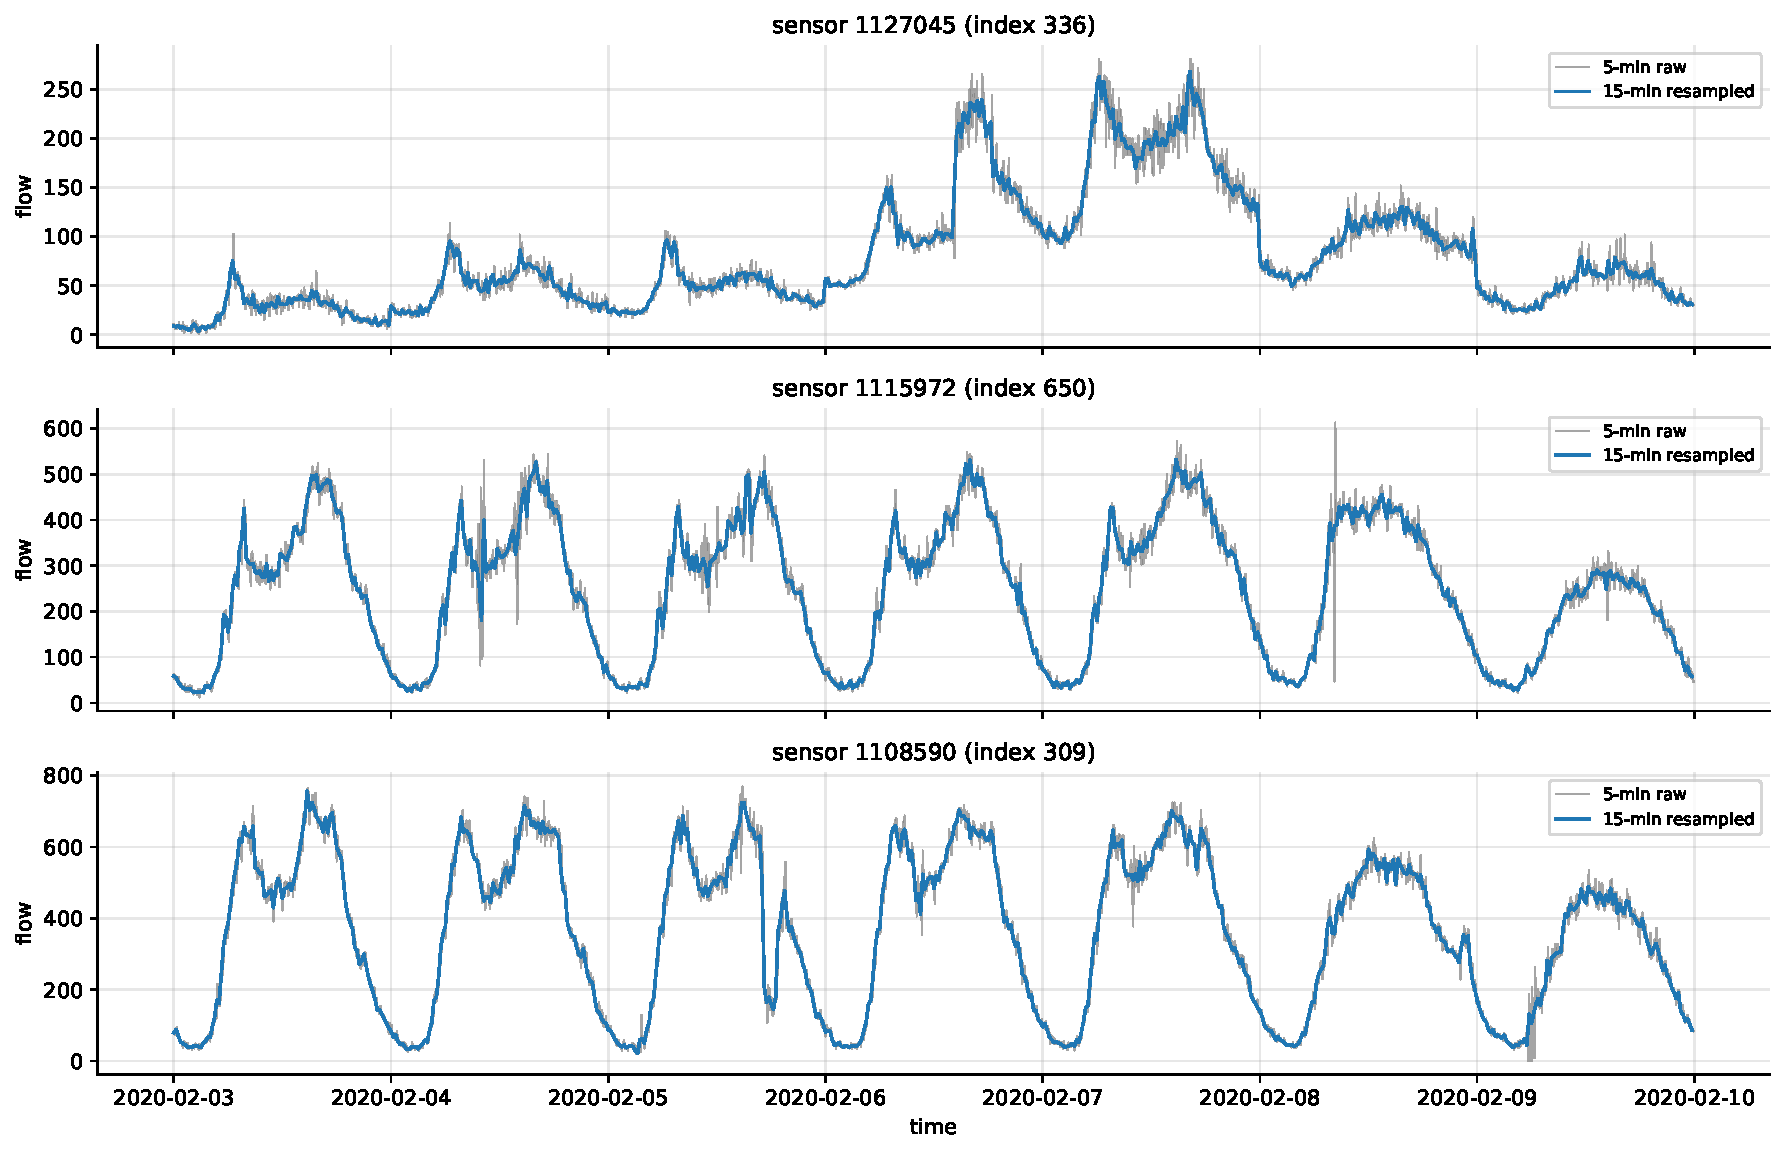
\includegraphics[width=\linewidth]{figures/fig_q3_week.pdf}
\caption{Flow for three sensors from 3 to 9 February 2020. The grey line is the raw 5-minute series and the blue line is the 15-minute average.}
\label{fig:q3week}
\end{figure}

\subsection*{Q3(b): Constructing the traffic graph}

The adjacency submatrix is taken from the LargeST road-network matrix using the row position of each San Diego sensor in the metadata. The flow columns are ordered by the same rows, so row $i$ of $A_{SD}$ and column $i$ of the flow tensor describe the same sensor. Table~\ref{tab:graph} reports the graph statistics and Figure~\ref{fig:q3graph} shows the matrix and the degree distribution.

\begin{table}[htbp]
\centering
\caption{Statistics of the San Diego road-distance adjacency $A_{SD}\in\mathbb{R}^{716\times716}$.}
\label{tab:graph}
\footnotesize
\begin{tabular}{lr}
\toprule
Quantity & Value \\
\midrule
Nodes & 716 \\
Nonzero entries, including the 716 diagonal entries & 18,035 \\
Nonzero directed edges, excluding self-loops & 17,319 \\
Density of off-diagonal entries & 3.38\% \\
Symmetric & No \\
Edges whose reverse edge also exists & 78.6\% \\
Edge weight range / mean & 0.010 to 1.000 / 0.297 \\
Out-degree mean / median / maximum & 24.2 / 20 / 70 \\
Isolated nodes / weakly connected components & 3 / 7 \\
Mean edge length (straight line) & 2.28 km \\
Correlation between edge weight and edge length & $-0.38$ \\
\bottomrule
\end{tabular}
\end{table}

\begin{figure}[htbp]
\centering
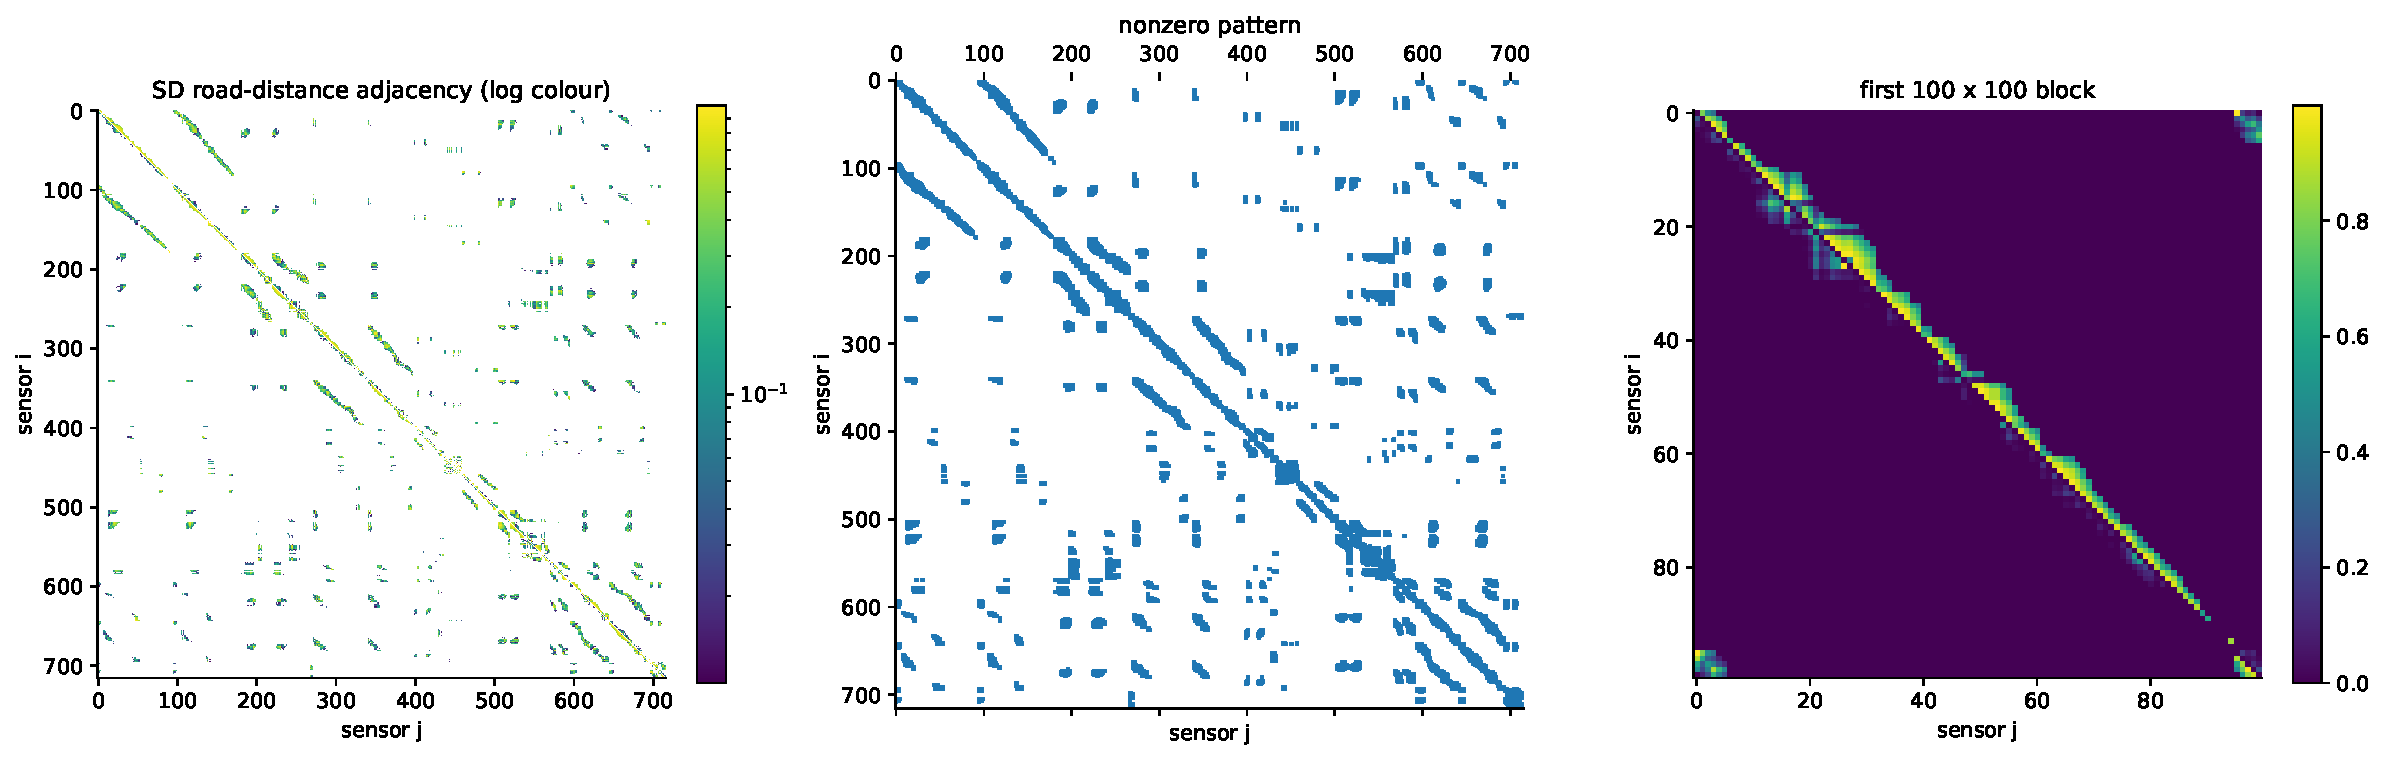
\includegraphics[width=\linewidth]{figures/fig_q3_adjacency.pdf}
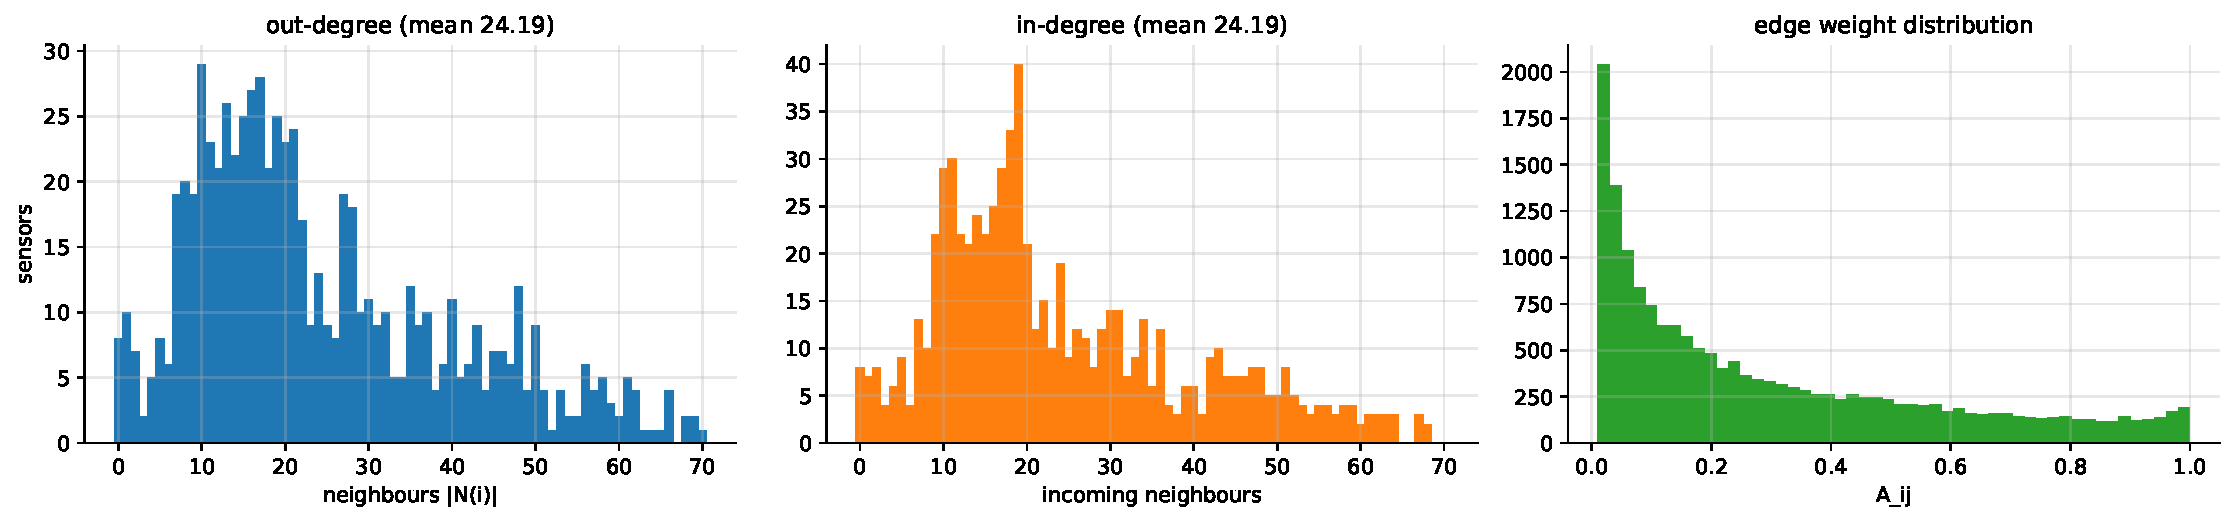
\includegraphics[width=\linewidth]{figures/fig_q3_degree.pdf}
\caption{Top: adjacency weights on a log colour scale, the nonzero pattern, and the first $100\times100$ block. Bottom: out-degree, in-degree, and edge-weight distributions.}
\label{fig:q3graph}
\end{figure}

A nonzero entry $A_{ij}$ means that sensor $j$ lies within the road-distance threshold of sensor $i$ on the road network. Its value decreases as the road distance grows, which is why the weights correlate negatively with edge length. The matrix is not symmetric because road distance depends on the direction of travel: about one fifth of the edges have no reverse edge. A nonzero entry is therefore a statement about proximity along the network, not about measured traffic interaction.

\subsection*{Q3(c): Graph neighbourhoods}

Sensor 1126411 (index 33) is chosen because its out-degree is close to the median. It has 20 one-hop neighbours between 0.2 and 3.7 km away, and 53 further sensors at exactly two hops, for 73 sensors within two hops.

\paragraph{Why neighbours help.}
Raw flow does not answer this question. Its correlation is about 0.8 for every hop distance because all sensors share the same daily cycle (Figure~\ref{fig:q3corr}, top). After removing each sensor's average weekly profile and the network-wide mean at each time step, the remaining local fluctuations show clear spatial structure. Across all sensor pairs, this local correlation is 0.20 at one hop, 0.10 at two hops, and 0.05 at three hops, and it is near zero beyond five hops. For sensor 33 it is 0.33 with one-hop neighbours, 0.31 with two-hop neighbours, and $-0.03$ with all other sensors. Neighbours therefore carry information about deviations from the usual pattern, such as a slowdown that is already visible upstream.

\begin{figure}[htbp]
\centering
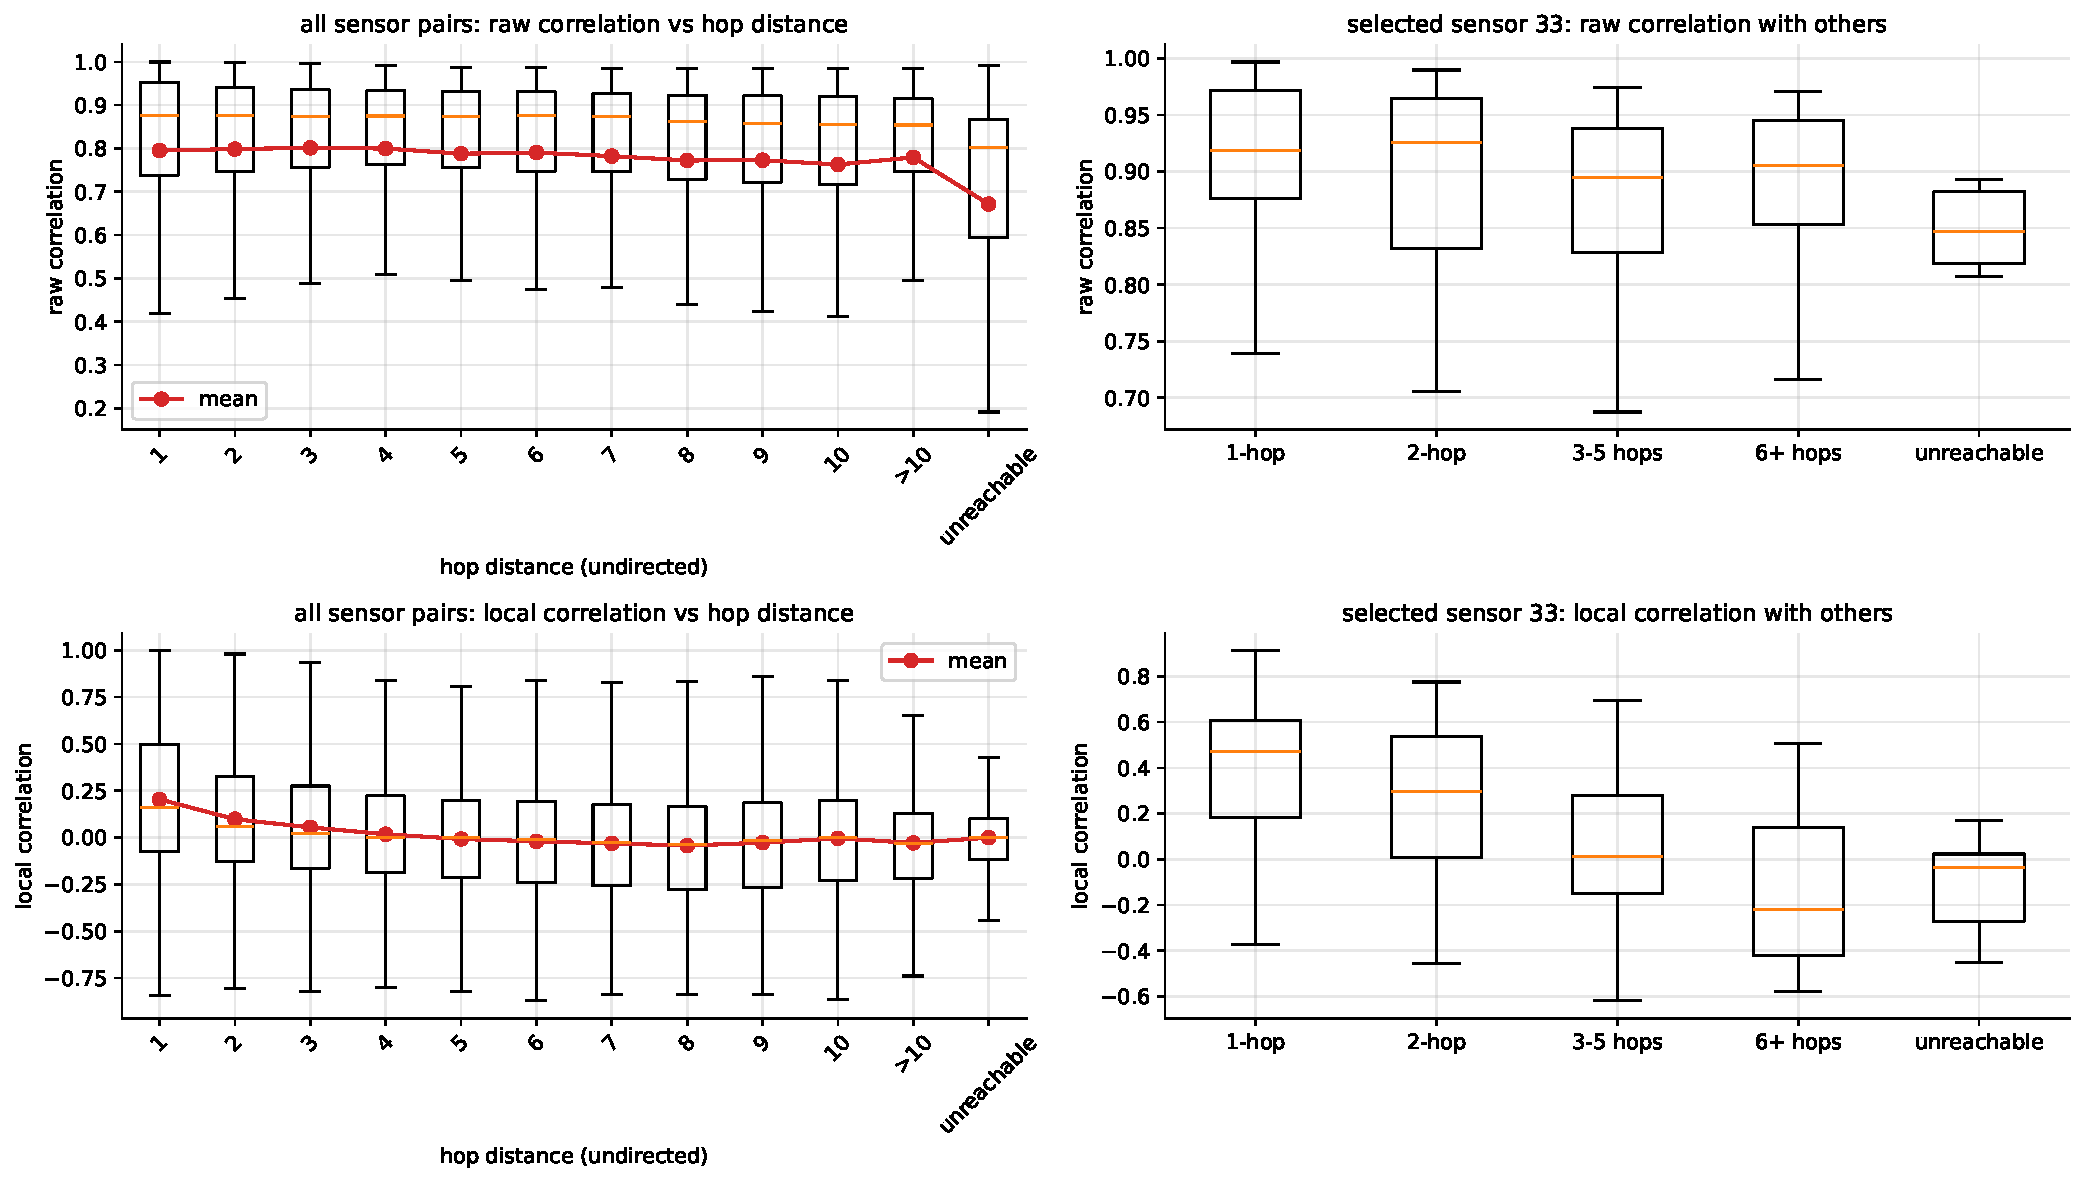
\includegraphics[width=\linewidth]{figures/fig_q3_correlation.pdf}
\caption{Correlation by hop distance for all sensor pairs (left) and for sensor 33 (right). Top: raw training flow. Bottom: local fluctuations after removing each sensor's weekly profile and the network-wide mean.}
\label{fig:q3corr}
\end{figure}

\paragraph{One-hop versus two-hop aggregation.}
One graph layer computes $\Ahat Z$, so each sensor combines only its direct neighbours. Two layers compute $\Ahat^2 Z$ through the intermediate features, so each sensor also receives neighbours of neighbours, with weights equal to products of normalised edge weights. Two-hop information is wider but weaker, and it passes through the intermediate sensors' representations rather than arriving directly.

\paragraph{Too many layers.}
Yes. Figure~\ref{fig:q3smooth} applies $\Ahat^k$ to one week of standardised training data. One propagation step raises the mean pairwise correlation between sensors from 0.84 to 0.95 and reduces the spread across sensors by 43\%. After 32 steps the spread is 0.36 of its original value. Each layer averages features, so deep stacks make sensors indistinguishable. Meanwhile, the receptive field grows from 3.4\pct of the network at one hop to 24\pct at four hops and 65\pct at ten hops, far beyond the two-hop range in which local correlation is still meaningful. Deep stacks would add mostly irrelevant, distant information and would remove the local differences that a forecast needs.

\begin{figure}[htbp]
\centering
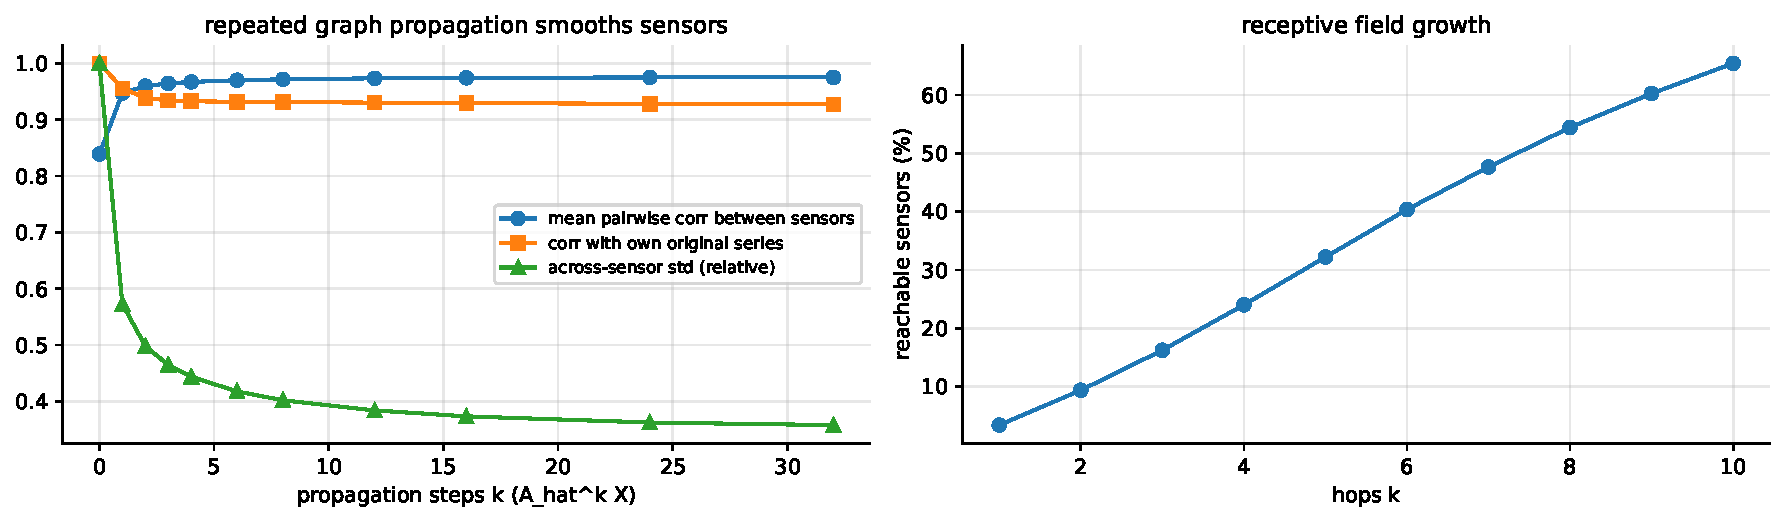
\includegraphics[width=\linewidth]{figures/fig_q3_oversmoothing.pdf}
\caption{Left: effect of repeated propagation $\Ahat^k X$ on one week of standardised training data. Right: fraction of sensors reachable within $k$ hops.}
\label{fig:q3smooth}
\end{figure}

\section{Spatio-Temporal Traffic Forecasting}
\label{sec:q4}

\subsection*{Q4(a): Forecasting windows}

Each sample uses $X_t=[x_{t-7},\ldots,x_t]$ and predicts $Y_t=[x_{t+1},\ldots,x_{t+4}]$, with $x_t\in\mathbb{R}^{716\times1}$. Training covers 2020, validation covers January to March 2021, and testing covers April to December 2021. Windows are built separately inside each split, so no input or target crosses a boundary. This gives 35,125 training, 8,629 validation, and 26,389 test windows. Flow is standardised with one mean and standard deviation, 202.46 and 161.26, computed from observed training values only.

\subsection*{Q4(b): Architecture}

\paragraph{Temporal encoder.}
Each sensor's eight inputs pass through two 1D convolutions shared across sensors: a kernel of size 3 with 32 output channels, then a kernel of size 3 with dilation 2. Both use padding that keeps eight time steps and are followed by ReLU. A linear layer maps the flattened $8\times32$ features to $d=32$, giving $Z\in\mathbb{R}^{B\times N\times32}$.

\paragraph{Graph convolution.}
The graph layer follows the graph convolution of \citet{kipf2017gcn}, computes the required operation, and adds it to its input,
\begin{equation}
  H=Z+\operatorname{ReLU}\!\left(\Ahat ZW_g\right),
\end{equation}
where the multiplication by $\Ahat$ acts on the node dimension of each batch item. The residual path was added after the first experiments. Without it, the forecast head saw only neighbour averages: in the row-normalised road graph a sensor keeps a median weight of 0.14 on itself, and the fixed-graph model reached a training MAE of 40.2, twice that of the temporal-only model. The residual path restores each sensor's own representation and leaves the graph term to add neighbour information.

\paragraph{Forecast head and training.}
After dropout of 0.1, a two-layer MLP with hidden size 32 outputs the four future values for every sensor. Predictions are converted back to flow units, and the loss is MAE computed only on observed targets. The temporal-only baseline in Q4(c) uses the same encoder, head, and residual graph layer with $\Ahat$ replaced by the identity, so it has the same 13,668 parameters as the fixed-graph model.

\subsection*{Q4(c): Temporal-only baseline}

Table~\ref{tab:results} reports all results; the fixed-graph model is discussed here. It lowers test MAE from 24.20 to 23.17 and RMSE from 35.68 to 34.33, with the same parameter count. The gain grows with the horizon: at 15 minutes the two models differ by 0.18 MAE, while at 60 minutes they differ by 1.84 (Table~\ref{tab:horizon}). The fixed graph improves 87.2\pct of sensors, and the improvement is larger for sensors with more neighbours (Spearman correlation 0.29 between out-degree and gain). Explicit spatial dependencies therefore improve accuracy, mainly at longer horizons, where a sensor's own recent history becomes less informative than conditions on nearby roads.

\section{Fixed versus Learnable Adjacency}
\label{sec:q5}

All three graph models use the encoder, graph layer, head, splits, and training protocol of Section~\ref{sec:q4}. Only $\Ahat$ changes.

\subsection*{Q5(a): Fixed adjacency}

$A_{SD}$ is directed, so the symmetric normalisation $D^{-1/2}(A+I)D^{-1/2}$ is not used. The diagonal of $A_{SD}$ is removed and replaced by the identity, and each row is divided by its sum:
\begin{equation}
  \Ahat_{\text{fixed}}=D^{-1}(A+I),\qquad D_{ii}=\textstyle\sum_j (A+I)_{ij}.
\end{equation}
Each sensor then takes a weighted average over itself and its out-neighbours, and every row sums to one. $\Ahat_{\text{fixed}}$ is stored as a buffer and does not change during training. Training took 249 s over 22 epochs; the test MAE is 23.17 and the RMSE is 34.33.

\subsection*{Q5(b): Learnable adjacency}

Two embedding matrices $E_1,E_2\in\mathbb{R}^{716\times10}$ are initialised from a standard normal distribution, and
\begin{equation}
  A_{\text{adaptive}}=\operatorname{Softmax}\!\left(\operatorname{ReLU}\!\left(E_1E_2^\top\right)\right)
\end{equation}
is applied row-wise, following Graph WaveNet~\citep{wu2019graphwavenet}. The full dense matrix is used without top-$k$ sparsification. Gradients reach $E_1$ and $E_2$ through every entry of the softmax. Two details were required for the learned graph to be meaningful.

\paragraph{No weight decay on the embeddings.}
In a first run, the weight decay of $10^{-4}$ also acted on $E_1$ and $E_2$. Their mean row norm fell from 3.1 to 0.12, so $E_1E_2^\top$ approached zero and every row of $A_{\text{adaptive}}$ became uniform at $1/716$. The model then averaged all sensors instead of learning a graph. Excluding the graph parameters from weight decay keeps the embedding norm near 3.1 and gives about 23 effective neighbours per sensor.

\paragraph{Never-observed sensors are not message sources.}
In a second run, the five strongest hubs of the learned graph were sensors that are never observed, and these 19 sensors received 17.4\pct of all learned weight. Their input is a constant fill value, so the model used them as a bias term rather than as neighbours. Their columns are now set to $-\infty$ before the softmax. The set is determined from training data only, and these sensors still receive forecasts.

With both changes, the adaptive model reaches a test MAE of 20.91 and an RMSE of 31.67, the best of all models, compared with 23.17 and 34.33 for the fixed graph. It has 27,988 parameters, of which 14,320 belong to the embeddings. Figure~\ref{fig:q5} compares the learned matrices with the fixed one.

\begin{figure}[htbp]
\centering
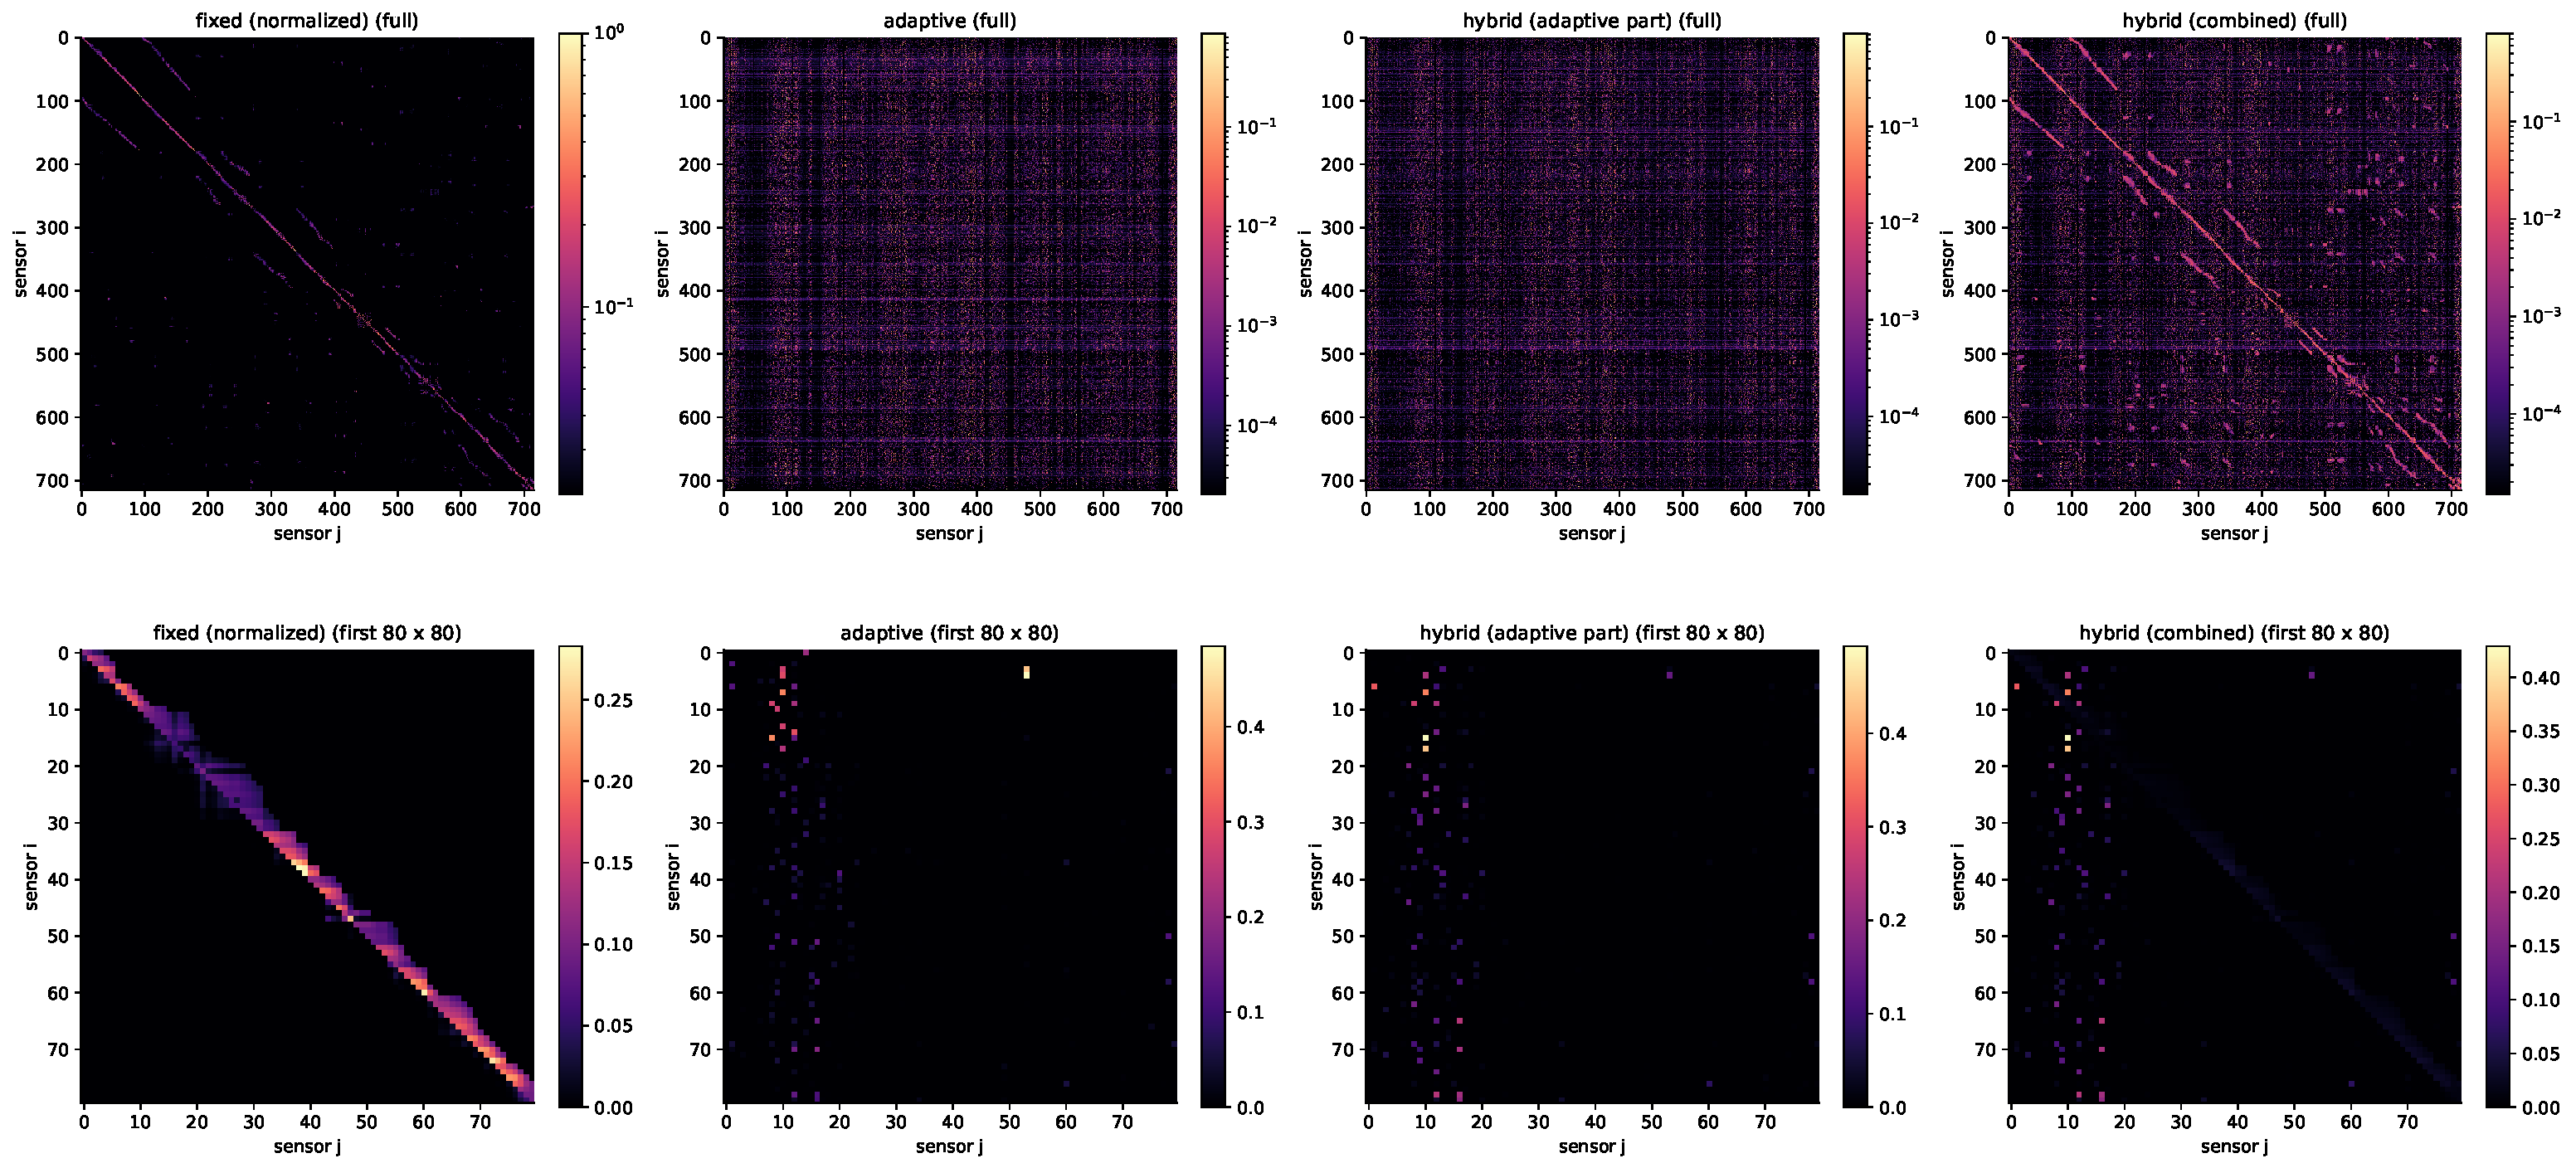
\includegraphics[width=\linewidth]{figures/fig_q5_adjacency.pdf}
\caption{Fixed, adaptive, and hybrid adjacency matrices. Top: full matrices on a log colour scale. Bottom: the first $80\times80$ block on a linear scale. The fixed graph is concentrated near the diagonal, while the learned graphs spread their weight over distant sensors.}
\label{fig:q5}
\end{figure}

\subsection*{Q5(c): Hybrid adjacency}

The hybrid graph is
\begin{equation}
  A_{\text{hybrid}}=\alpha\,\Ahat_{\text{fixed}}+(1-\alpha)\,A_{\text{adaptive}},\qquad \alpha=\sigma(\theta),
\end{equation}
with $\theta$ initialised at zero so that $\alpha$ starts at 0.5. Both components are row-normalised, so both are row-stochastic and the combination is also row-stochastic. The learned $\alpha$ fell to 0.13 at the selected epoch and to 0.03 by the end of training, so the model chose to rely almost entirely on the learned component. The hybrid model reaches a test MAE of 21.73 and an RMSE of 32.77. It improves on the fixed graph but not on the adaptive graph.

\section{Experimental Analysis and Interpretation}
\label{sec:q6}

\subsection*{Q6(a): Forecasting comparison}

\begin{table}[htbp]
\centering
\caption{Test results in original flow units. MAPE uses targets above 10. Validation MAE is included because it selects the checkpoint. Training time is the wall-clock time of all epochs, including validation.}
\label{tab:results}
\footnotesize
\begin{adjustbox}{max width=\linewidth}
\begin{tabular}{llrrrrrrr}
\toprule
Model & Adjacency & MAE & RMSE & MAPE (\%) & Val MAE & Training time (s) & Epochs & Parameters \\
\midrule
Temporal-only & None & 24.20 & 35.68 & 18.64 & 22.24 & 206.0 & 20 & 13,668 \\
STGNN & Fixed & 23.17 & 34.33 & 17.14 & 21.07 & 249.2 & 22 & 13,668 \\
STGNN & Adaptive & \textbf{20.91} & \textbf{31.67} & \textbf{13.71} & \textbf{18.08} & 234.4 & 20 & 27,988 \\
STGNN & Hybrid & 21.73 & 32.77 & 13.98 & 19.09 & 173.5 & 15 & 27,989 \\
\bottomrule
\end{tabular}
\end{adjustbox}
\end{table}

\begin{table}[htbp]
\centering
\caption{Test MAE and RMSE by forecast horizon.}
\label{tab:horizon}
\footnotesize
\begin{tabular}{lrrrrrrrr}
\toprule
 & \multicolumn{2}{c}{15 min} & \multicolumn{2}{c}{30 min} & \multicolumn{2}{c}{45 min} & \multicolumn{2}{c}{60 min} \\
\cmidrule(lr){2-3}\cmidrule(lr){4-5}\cmidrule(lr){6-7}\cmidrule(lr){8-9}
Model & MAE & RMSE & MAE & RMSE & MAE & RMSE & MAE & RMSE \\
\midrule
Temporal-only & 18.52 & 25.46 & 22.49 & 32.31 & 26.04 & 38.21 & 29.75 & 44.05 \\
Fixed & 18.34 & 25.42 & 21.84 & 31.75 & 24.57 & 36.52 & 27.91 & 41.54 \\
Adaptive & \textbf{17.11} & \textbf{24.57} & \textbf{19.75} & \textbf{29.55} & \textbf{22.24} & \textbf{33.79} & \textbf{24.55} & \textbf{37.31} \\
Hybrid & 17.37 & 25.31 & 20.43 & 30.42 & 23.31 & 35.07 & 25.80 & 38.70 \\
\bottomrule
\end{tabular}
\end{table}

Every graph model improves on the temporal-only baseline, by 4.3\pct for the fixed graph, 13.6\pct for the adaptive graph, and 10.2\pct for the hybrid graph in MAE. Error grows with the horizon for every model, and the gap between models grows with it. Training costs are similar because the graph multiplication over 716 sensors is small next to the temporal encoder, which processes every sensor separately. Figure~\ref{fig:q6pred} shows that all models follow the daily shape of three test sensors. The visible differences are at peaks and rapid changes, where the 60-minute forecasts lag the observed flow.

\begin{figure}[htbp]
\centering
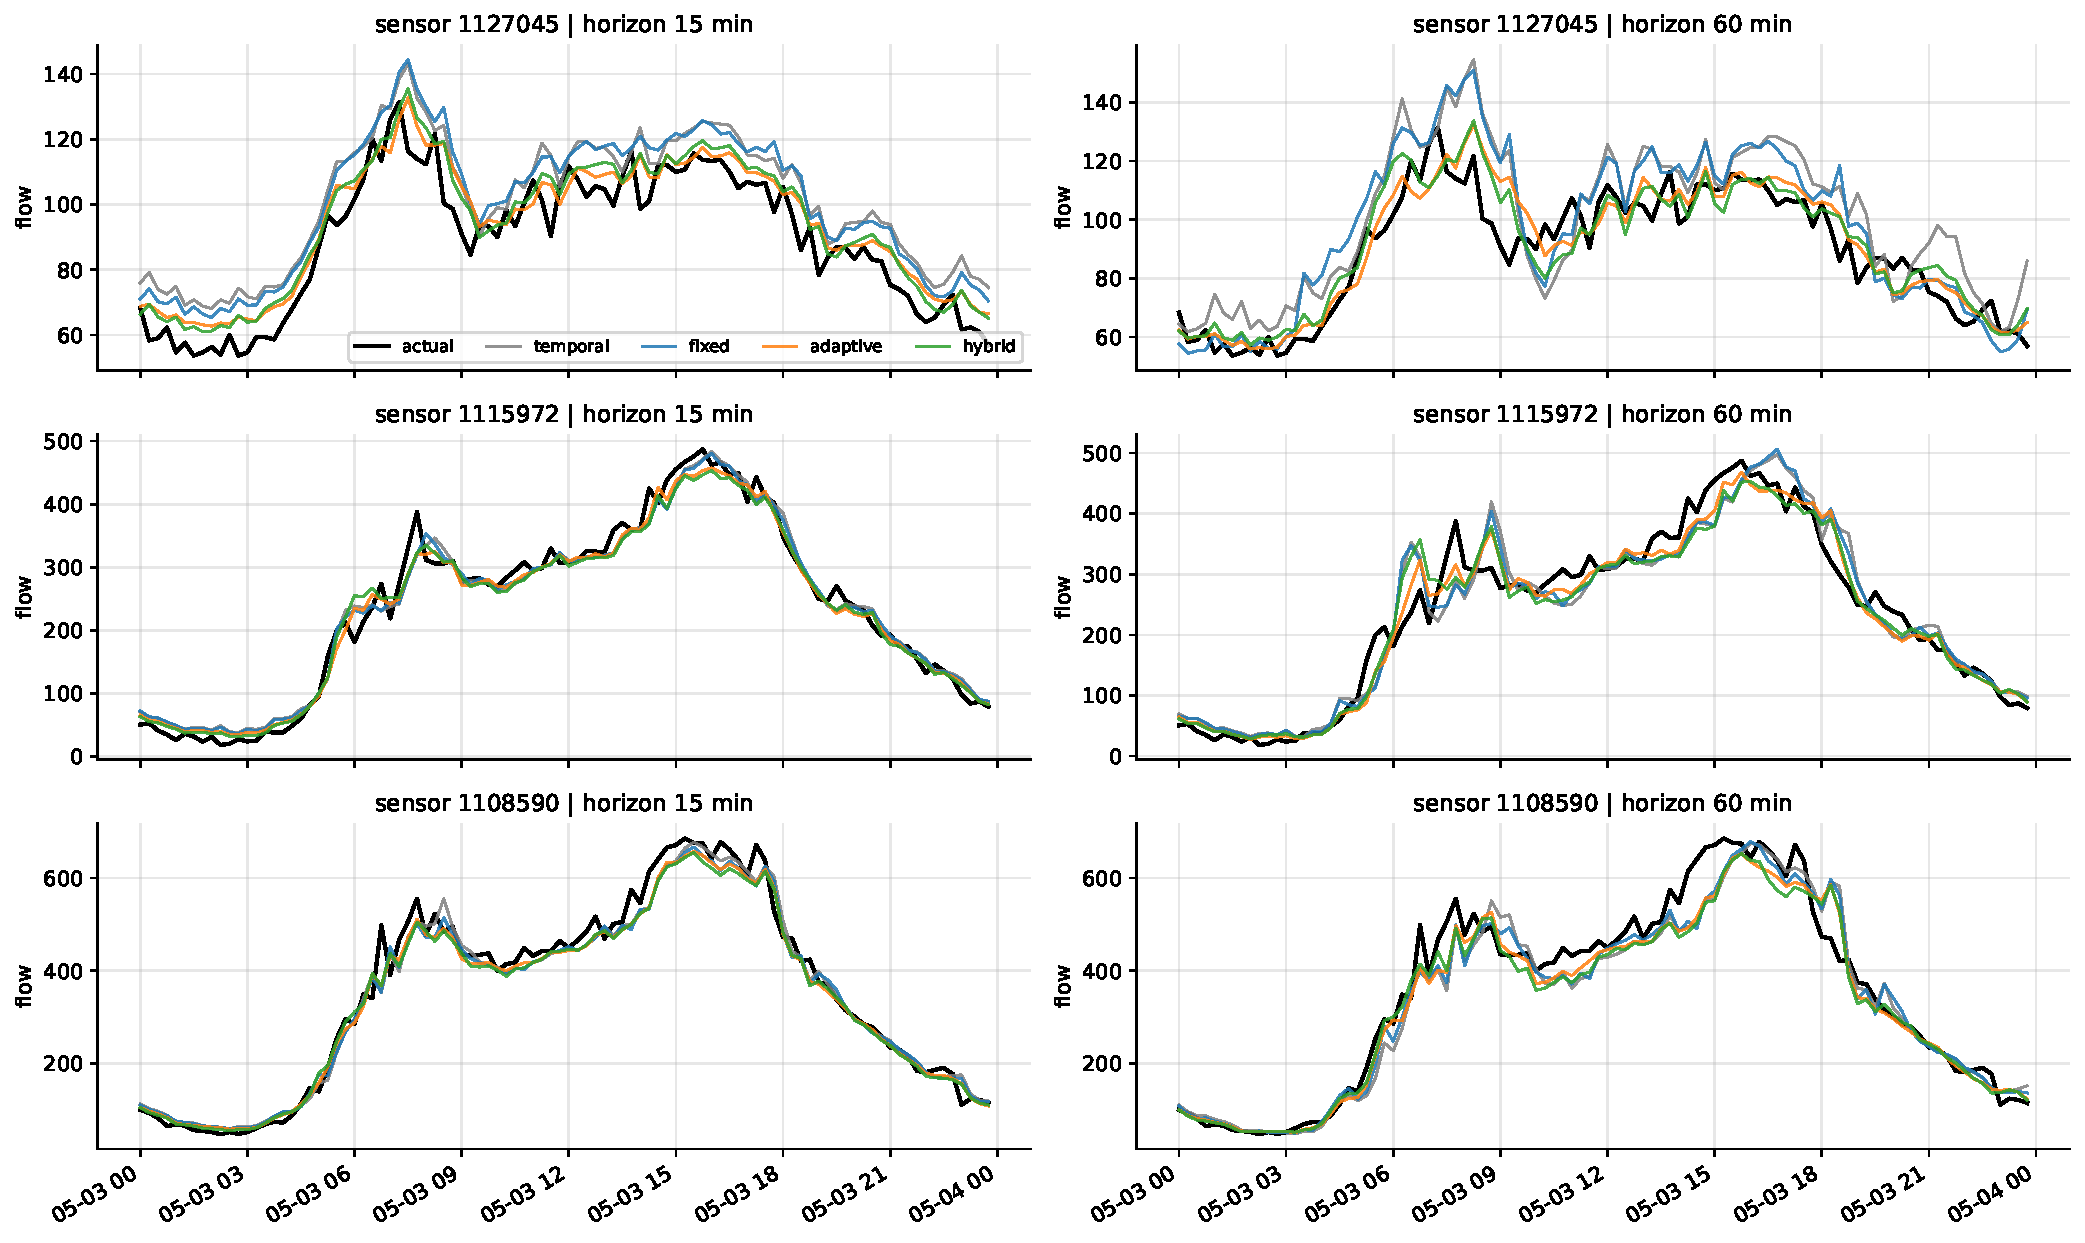
\includegraphics[width=\linewidth]{figures/fig_q6_predictions.pdf}
\caption{Predicted and actual flow for three test sensors on 3 May 2021, at the 15-minute (left) and 60-minute (right) horizons.}
\label{fig:q6pred}
\end{figure}

\subsection*{Q6(b): Graph structure analysis}

The analysis uses the 697 sensors observed during training. A road edge is counted in either direction, local correlation is the quantity defined in Q3(c), and all distances are straight-line distances. Table~\ref{tab:learned} and Figure~\ref{fig:q6learned} summarise the comparison.

\begin{table}[htbp]
\centering
\caption{Learned top-$k$ neighbours compared with road edges and random sensor pairs.}
\label{tab:learned}
\footnotesize
\begin{tabular}{lrrr}
\toprule
Neighbour set & Road edge & Mean distance (km) & Local correlation \\
\midrule
Random pair & 4.1\% & 27.1 & 0.002 \\
Road edge & 100\% & 2.4 & 0.216 \\
Adaptive, strongest neighbour & 6.3\% & 26.6 & 0.248 \\
Adaptive, top 10 & 4.4\% & 27.8 & 0.086 \\
Hybrid (learned part), strongest neighbour & 4.9\% & 29.1 & 0.279 \\
Hybrid (learned part), top 10 & 3.5\% & 29.2 & 0.084 \\
\bottomrule
\end{tabular}
\end{table}

\paragraph{1. Are the strongest learned connections in the road graph?}
No. The strongest learned neighbour of a sensor is a road neighbour 6.3\pct of the time, and the ten strongest are road neighbours 4.4\pct of the time. A random sensor pair is a road edge 4.1\pct of the time. The learned graph therefore does not rediscover the road graph.

\paragraph{2. Are learned connections geographically close?}
No. The ten strongest learned neighbours lie 27.8 km away on average, while random pairs lie 27.1 km apart and road neighbours lie 2.4 km apart. The Spearman correlation between learned weight and distance is $-0.001$. Figure~\ref{fig:q6learned} (right) shows that the strongest learned links cross the whole region.

\paragraph{3. Does the learned graph capture dependencies absent from the road graph?}
Partly. The strongest learned neighbour has a local correlation of 0.25, which exceeds that of an average road neighbour (0.22) and is far above that of random pairs (0.002). In 7.5\pct of sensors, this neighbour cannot be reached at all through the road graph. The model has found sensors whose deviations move together even though no road connects them closely. The evidence is limited to the strongest links: the ten strongest learned neighbours have a local correlation of only 0.09, and they overlap with the ten most correlated sensors in only 2.6\pct of cases.

\paragraph{4. Why might a learned adjacency perform better or worse?}
It can perform better because it is optimised for the forecasting loss rather than for proximity. It can link sensors on related commuting routes, and several sensors share the same strongest neighbour (up to 27 sensors per target), so part of the learned graph acts as a shared summary of network-wide conditions. It can perform worse because it doubles the number of parameters, it must be learned from one year of data, and it has no physical prior to fall back on when the data are noisy or when conditions drift between years. It is also harder to interpret, as items 1 and 2 show.

\begin{figure}[htbp]
\centering
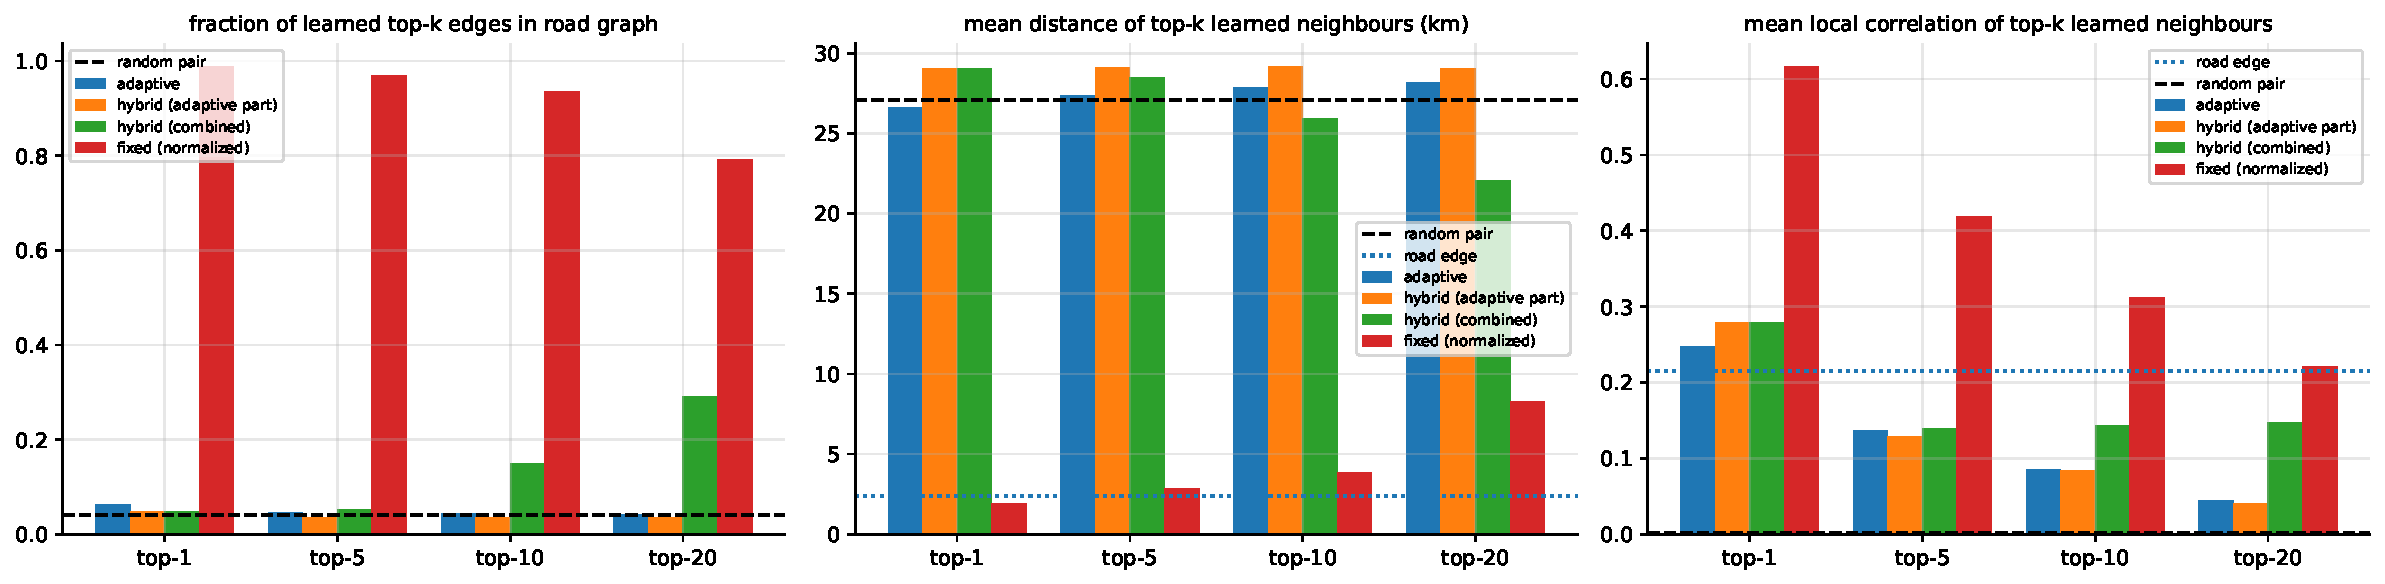
\includegraphics[width=\linewidth]{figures/fig_q6_learned_vs_road.pdf}
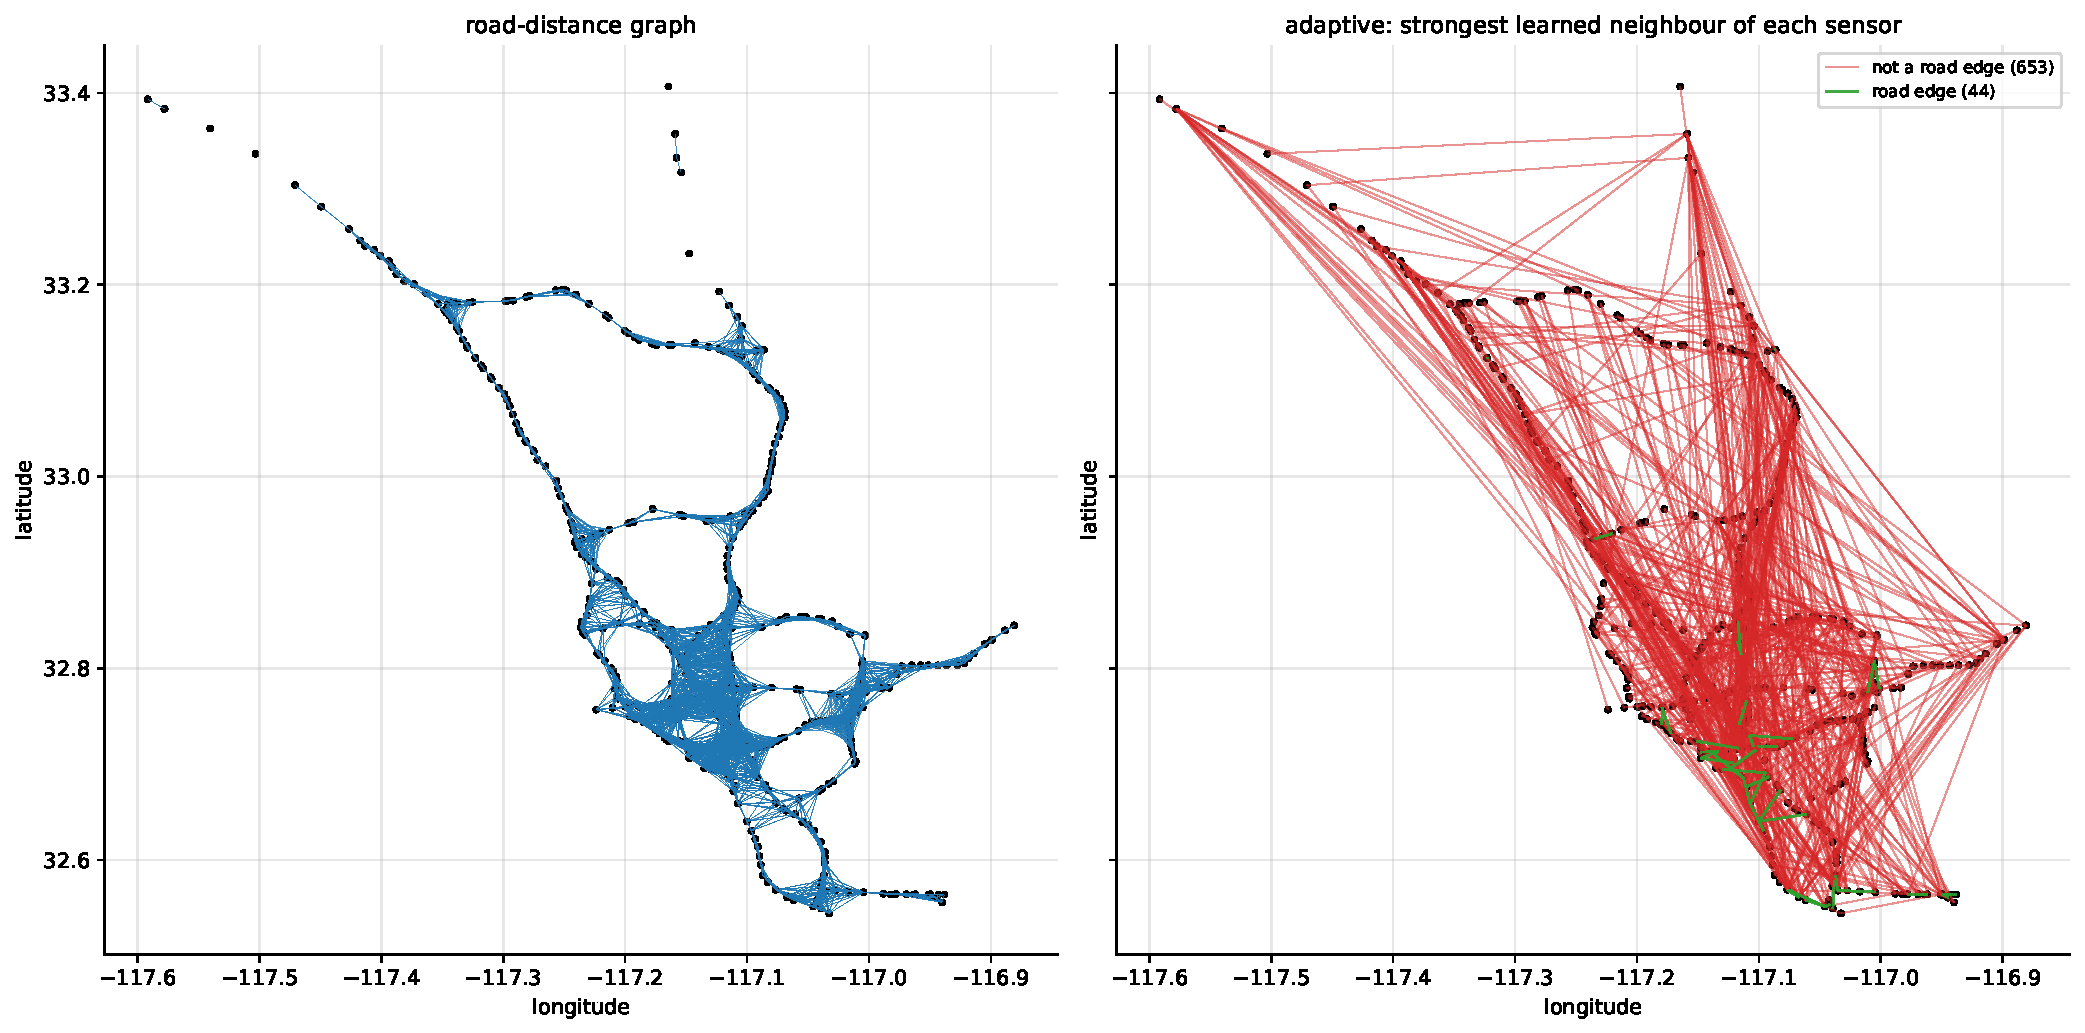
\includegraphics[width=0.92\linewidth]{figures/fig_q6_learned_map.pdf}
\caption{Top: fraction of learned top-$k$ neighbours that are road edges, their mean distance, and their mean local correlation. Bottom: the road graph (left) and the strongest learned neighbour of each sensor in the adaptive graph (right), coloured by whether the link is a road edge.}
\label{fig:q6learned}
\end{figure}

\subsection*{Q6(c): Critical discussion}

\paragraph{Does lower error imply real road connectivity?}
No. The adaptive model has the lowest error and the least road-like graph. The learned matrix is whatever combination of sensors reduces the loss. It can exploit correlated behaviour, shared network-wide conditions, or simple regularities of the data, none of which require a physical road link. Forecast accuracy measures predictive usefulness, not structural correctness.

\paragraph{Why might a hybrid graph outperform either alone?}
The fixed graph supplies a reliable local prior: short-range propagation along roads, available from the first epoch and robust to noise. The learned graph supplies long-range dependencies that the road graph cannot represent. A combination can use both and can fall back on the road graph where the learned part is poorly estimated. In this experiment the hybrid did not outperform the adaptive graph. The learned $\alpha$ moved towards the learned component, so the two models became similar, and their validation MAE differs by about one unit, which is within the epoch-to-epoch variation of these runs.

\paragraph{Limitations of a static graph.}
Figure~\ref{fig:q6hour} shows that the benefit of the graph changes during the day. The adaptive graph lowers MAE by 29 to 32\pct between midnight and 03:00 and by 19\pct at 08:00, but it is 1 to 3\pct worse than the temporal-only model between 15:00 and 17:00. The hybrid graph is worse than the temporal-only model from 12:00 to 17:00, by up to 12\pct at 16:00. One static matrix must average over regimes in which different sensors interact: free flow at night, directional peaks in the morning and evening, and incidents that change interactions within minutes. A time-dependent or input-dependent adjacency would be required to represent these changes.

\begin{figure}[htbp]
\centering
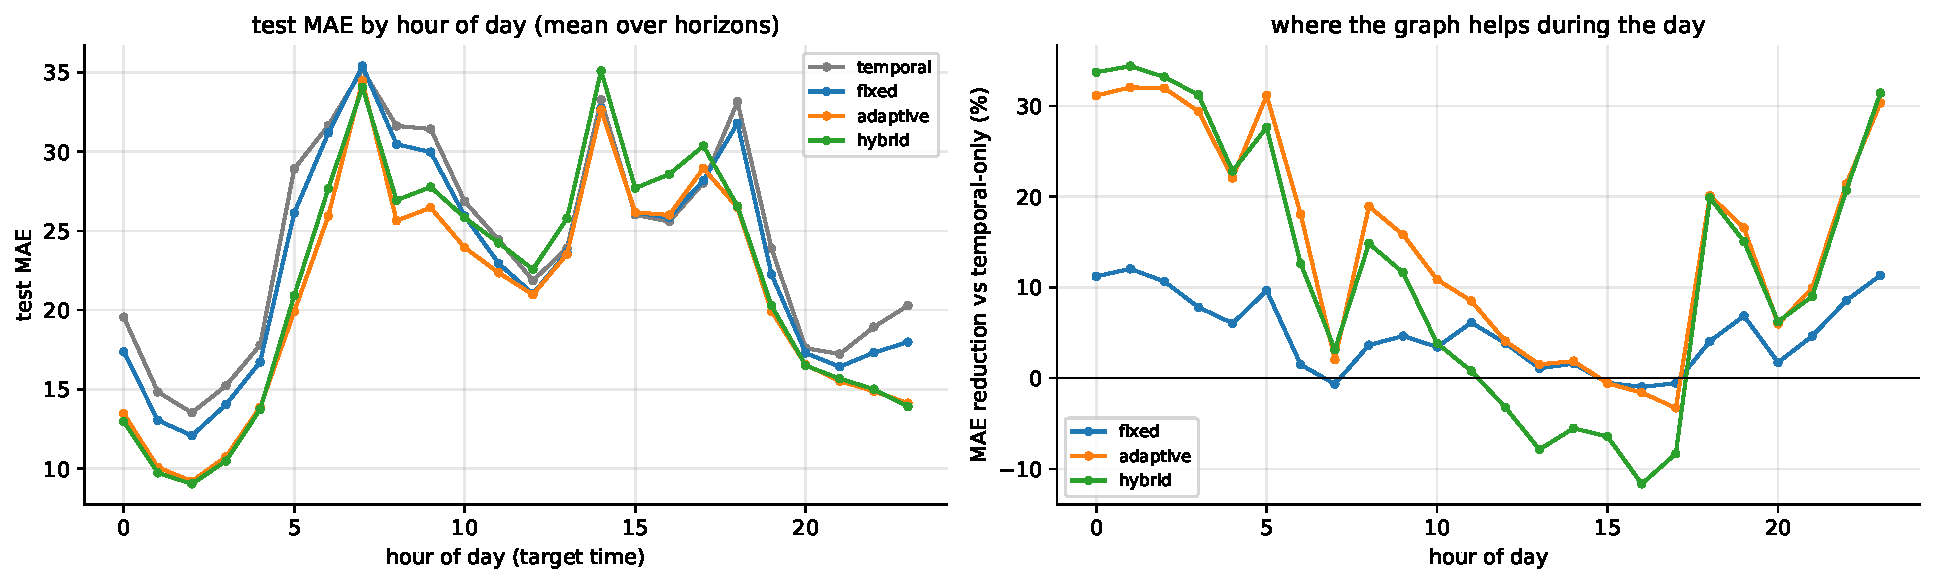
\includegraphics[width=\linewidth]{figures/fig_q6_hour.pdf}
\caption{Test MAE by hour of the target time, averaged over horizons (left), and MAE reduction relative to the temporal-only model (right).}
\label{fig:q6hour}
\end{figure}

\section{Reproducibility}
\label{sec:q7}

Table~\ref{tab:config} lists the training configuration, which is identical for all four models. Each experiment saves a resumable checkpoint every two epochs and whenever validation improves. The test metrics use the checkpoint with the lowest validation MAE.

\begin{table}[htbp]
\centering
\caption{Training configuration and hardware.}
\label{tab:config}
\footnotesize
\begin{tabular}{ll}
\toprule
Setting & Value \\
\midrule
Optimiser & Adam, learning rate $10^{-3}$ \\
Weight decay & $10^{-4}$, not applied to $E_1$, $E_2$, or $\theta$ \\
Batch size & 64 \\
Maximum epochs / early stopping & 50 / patience 10 on validation MAE \\
Gradient clipping & norm 5 \\
Hidden size $d$ / embedding size $d_e$ / dropout & 32 / 10 / 0.1 \\
Graph layers & 1 \\
Loss & masked MAE in flow units \\
Random seed & 42 \\
\midrule
GPU & NVIDIA GeForce RTX 4050 Laptop, 6 GB \\
CPU / memory & Intel Core, 14 cores and 20 threads / 15.7 GB \\
Software & Python 3.11, PyTorch 2.5.1, CUDA 12.4 \\
Time per epoch & 10.3 to 11.7 s; peak GPU memory 0.82 GB \\
\bottomrule
\end{tabular}
\end{table}

The source code is organised as one script per question. The data scripts download and resample LargeST and build the graph statistics, \texttt{run\_experiment.py} trains one model with \texttt{-{}-model} set to \texttt{temporal}, \texttt{fixed}, \texttt{adaptive}, or \texttt{hybrid}, and \texttt{analyze.py} produces every table and figure in Questions 5 and 6. The code is available at \url{https://github.com/syeddaniyalg/cs434-pa3}, and its README lists the exact commands.

\section{Limitations}

All forecasting results come from one seed. Validation MAE varies by about 1.5 between consecutive epochs, so differences of this size, such as adaptive against hybrid, are not conclusive. The training year 2020 contains the COVID-19 traffic reduction, and the 2021 test period differs from it; test errors are 2 to 3 MAE above validation errors for every model. The models use flow only, without time-of-day features, and a single graph layer. The learned graph depends on its random initialisation, so its specific edges are not reproducible across seeds even if its statistics are. The Question 1 and 2 results are exact but concern idealised examples.

\section{Conclusion}

The small examples show that a graph layer is limited by what its aggregation keeps and by whether it can tell directions apart. On LargeST-SD, adding the road graph lowers test MAE by 4.3\pct over a temporal-only model with the same parameters, and a learned graph lowers it by 13.6\%. The learned graph is not a map of the road network: its links ignore distance but connect sensors with correlated fluctuations. The comparisons were valid only after the graph layer kept each sensor's own signal and after the learned graph was protected from weight decay and from never-observed sensors. A static graph of either kind still cannot represent interactions that change during the day.

\begin{thebibliography}{3}

\bibitem[Kipf and Welling(2017)]{kipf2017gcn}
Thomas N. Kipf and Max Welling.
\newblock Semi-supervised classification with graph convolutional networks.
\newblock In \emph{International Conference on Learning Representations}, 2017.

\bibitem[Liu et~al.(2023)]{liu2023largest}
Xu Liu, Yutong Xia, Yuxuan Liang, Junfeng Hu, Yiwei Wang, Lei Bai, Chao Huang, Zhenguang Liu, Bryan Hooi, and Roger Zimmermann.
\newblock LargeST: A benchmark dataset for large-scale traffic forecasting.
\newblock In \emph{Advances in Neural Information Processing Systems, Datasets and Benchmarks Track}, volume 36, 2023.

\bibitem[Wu et~al.(2019)]{wu2019graphwavenet}
Zonghan Wu, Shirui Pan, Guodong Long, Jing Jiang, and Chengqi Zhang.
\newblock Graph WaveNet for deep spatial-temporal graph modeling.
\newblock In \emph{International Joint Conference on Artificial Intelligence}, pages 1907--1913, 2019.

\end{thebibliography}

\end{document}
